%\begin{name}
%	{Thầy Nguyễn Bình Nguyên}
%	{24-26-2-HaNoi-ChuyenKNTN-lan1}
%\end{name}
\section{Chuyên KNTN - Lần 1 -- NH: 25-26}
\setcounter{ex}{0}
\Opensolutionfile{ans}[ans/ans-2-TT-HaNoi-ChuyenKHTN-lan1]
\caulc
\begin{ex}%[2-TT-HaNoi-ChuyenKNTN-lan1]%[Nguyễn Bình Nguyên, 26-2-DuAnDeTHPT2025-2026]%[2H5N2-2]
	Trong không gian $Oxyz$, điểm nào sau đây thuộc đường thẳng $d \colon \dfrac{x-1}{1} = \dfrac{y-1}{1} = \dfrac{z-3}{2}$?
	\choice
	{$M(-1;-1;-3)$}
	{$N(1;1;2)$}
	{$P(-1;-1;-2)$}
	{\True $Q(1;1;3)$}
	\loigiai{
		Để kiểm tra một điểm có thuộc đường thẳng $d$ hay không, ta thay tọa độ của điểm đó vào phương trình của đường thẳng $d$.\\
		Thay tọa độ điểm $Q(1;1;3)$ vào $d$, ta được $\dfrac{1-1}{1} = \dfrac{1-1}{1} = \dfrac{3-3}{2} = 0$.
		Suy ra $Q \in d$.
	}
\end{ex}

\begin{ex}%[2-TT-HaNoi-ChuyenKNTN-lan1]%[Nguyễn Bình Nguyên, 26-2-DuAnDeTHPT2025-2026]%[1D6N4-2]
	Nghiệm của phương trình $2^{x+1} = 16$ là
	\choice
	{$x = 9$}
	{$x = 5$}
	{\True $x = 3$}
	{$x = 7$}
	\loigiai{
		Ta có $2^{x+1} = 16 \Leftrightarrow 2^{x+1} = 2^4\Leftrightarrow x = 3$.\\
		Vậy phương trình có nghiệm là $x = 3$.
	}
\end{ex}

\begin{ex}%[2-TT-HaNoi-ChuyenKNTN-lan1]%[Nguyễn Bình Nguyên, 26-2-DuAnDeTHPT2025-2026]%[2D1N1-2]
	Cho hàm số $f(x)$ có bảng biến thiên như sau:
	\begin{center}
		
\begin{tikzpicture}
			\tkzTabInit[lgt=1.5,espcl=2.5]
			{$x$ /1, $f'(x)$ /1, $f(x)$ /2.5}
			{$-\infty$, $-1$, $2$, $+\infty$}
			\tkzTabLine{, +, 0, -, 0, +, }
			\tkzTabVar{-/ $-\infty$, +/ $0$, -/ $-2$, +/ $+\infty$}
		\end{tikzpicture}
	\end{center}
	Hàm số đã cho nghịch biến trên khoảng nào dưới đây?
	\choice
	{$(-2;0)$}
	{\True $(-1;2)$}
	{$(-\infty;-1)$}
	{$(2;+\infty)$}
	\loigiai{
		Dựa vào bảng biến thiên, ta thấy đạo hàm $f'(x) < 0$ trên khoảng $(-1;2)$ và mũi tên của hàm số $f(x)$ đi xuống.\\
		Do đó, hàm số đã cho nghịch biến trên khoảng $(-1;2)$.
	}
\end{ex}

\begin{ex}%[2-TT-HaNoi-ChuyenKNTN-lan1]%[Nguyễn Bình Nguyên, 26-2-DuAnDeTHPT2025-2026]%[2H2N2-2]
	Trong không gian $Oxyz$, cho hai điểm $A(1;-2;-1)$ và $B(3;4;-3)$.
	Trung điểm của đoạn thẳng $AB$ có tọa độ là
	\choice
	{$(1;3;-1)$}
	{\True $(2;1;-2)$}
	{$(2;1;-12)$}
	{$(2;-1;-2)$}
	\loigiai{
		Gọi $I(x_I; y_I; z_I)$ là trung điểm của đoạn thẳng $AB$.\\
		Tọa độ điểm $I$ được tính theo công thức:
		$$\heva{&x_I = \dfrac{x_A + x_B}{2} = \dfrac{1 + 3}{2} = 2\\&y_I = \dfrac{y_A + y_B}{2} = \dfrac{-2 + 4}{2} = 1\\&z_I = \dfrac{z_A + z_B}{2} = \dfrac{-1 + (-3)}{2} = -2.}$$
		Vậy trung điểm của đoạn thẳng $AB$ có tọa độ là $(2;1;-2)$.
	}
\end{ex}

\begin{ex}%[2-TT-HaNoi-ChuyenKNTN-lan1]%[Nguyễn Bình Nguyên, 26-2-DuAnDeTHPT2025-2026]%[2D1N4-1]
	Đồ thị của hàm số $y = \dfrac{x+2}{x-2}$ có tiệm cận ngang là
	\choice
	{$x = 2$}
	{$x = -2$}
	{\True $y = 1$}
	{$y = -1$}
	\loigiai{
		Tập xác định: $\mathscr{D} = \mathbb{R} \setminus \{2\}$.\\
		Ta có $\lim\limits_{x \to +\infty} y = \lim\limits_{x \to +\infty} \dfrac{x+2}{x-2} = 1$ và $\lim\limits_{x \to -\infty} y = \lim\limits_{x \to -\infty} \dfrac{x+2}{x-2} = 1$.\\
		Vậy đường thẳng $y = 1$ là đường tiệm cận ngang của đồ thị hàm số.
	}
\end{ex}

\begin{ex}%[2-TT-HaNoi-ChuyenKNTN-lan1]%[Nguyễn Bình Nguyên, 26-2-DuAnDeTHPT2025-2026]%[2D1H5-1]
	\immini{
		Hàm số nào dưới đây có đồ thị là đường cong trong hình bên?
		\choice
		{$y = -x^2+2x-2$}
		{$y = x^2-2x-2$}
		{\True $y = -x^3+3x^2-2$}
		{$y = x^3-3x^2-2$}
	}{
		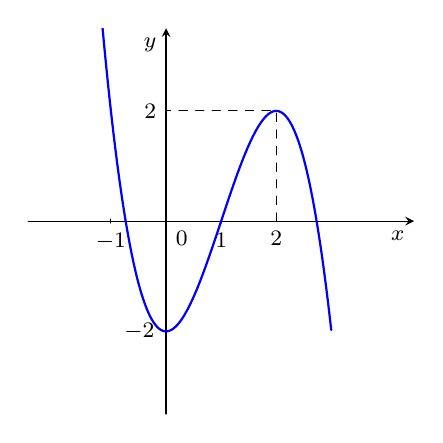
\begin{tikzpicture}[font=\footnotesize, line join=round, line cap=round, >=stealth, scale=0.7]
			\draw[->] (-2.5,0)--(4.5,0) node[below left] {$x$};
			\draw[->] (0,-3.5)--(0,3.5) node[below left] {$y$};
			\draw (0,0) node [below right] {$0$};
			\foreach \x in {-1,1} \draw[thin] (\x,1pt)--(\x,-1pt) node [below] {$\x$};
			\foreach \y in {-2} \draw[thin] (1pt,\y)--(-1pt,\y) node [left] {$\y$};
			\begin{scope}
				\clip (-2.5,-3.5) rectangle (4.5,3.5);
				\draw[blue, thick, samples=200, domain=-1.5:3, smooth, variable=\x] plot (\x, {-(\x)^3 + 3*(\x)^2 - 2});
			\end{scope}
			\draw[dashed](2,0)node[below]{$2$}--(2,2)--(0,2)node[left]{$2$};
		\end{tikzpicture}
	}
	\loigiai{
		Quan sát đồ thị ta thấy đây là đồ thị của hàm số bậc ba $y = ax^3 + bx^2 + cx + d$ có dạng chữ "N" ngược.\\
		Nhánh bên phải cùng của đồ thị hướng xuống dưới, suy ra hệ số $a < 0$.
		Do đó, ta loại phương án $y = x^2-2x-2$ và $y = x^3-3x^2-2$.\\
		Đồ thị hàm số đi qua điểm $(0; -2)$ và điểm $(2; 2)$.\\
		Xét phương án C: $y = -x^3+3x^2-2$.
		Ta có $y(2) = -2^3 + 3 \cdot 2^2 - 2 = -8 + 12 - 2 = 2$ (thỏa mãn).\\
		Hơn nữa, đạo hàm $y' = -3x^2 + 6x$.
		$y' = 0 \Leftrightarrow \hoac{&x=0\\&x=2}$, tương ứng với hai điểm cực trị của đồ thị là $(0; -2)$ và $(2; 2)$.
		Điều này hoàn toàn khớp với hình vẽ.\\
		Vậy hàm số cần tìm là $y = -x^3+3x^2-2$.
	}
\end{ex}

\begin{ex}%[2-TT-HaNoi-ChuyenKNTN-lan1]%[Nguyễn Bình Nguyên, 26-2-DuAnDeTHPT2025-2026]%[1D1H5-3]
	Trong khoảng $(0; 2\pi)$, phương trình $2\sin x = 1$ có bao nhiêu nghiệm?
	\choice
	{$1$}
	{\True $2$}
	{$3$}
	{$4$}
	\loigiai{
		Ta có phương trình $2\sin x = 1 \Leftrightarrow \sin x = \dfrac{1}{2} \Leftrightarrow \hoac{&x = \dfrac{\pi}{6} + k2\pi\\&x = \dfrac{5\pi}{6} + k2\pi} \quad (k \in \mathbb{Z})$.\\
		Vì ta chỉ xét nghiệm trên khoảng $(0; 2\pi)$ nên ta có:\\
		+ Trường hợp 1: $0 < \dfrac{\pi}{6} + k2\pi < 2\pi \Leftrightarrow -\dfrac{1}{12} < k < \dfrac{11}{12}$.
		Do $k \in \mathbb{Z}$ nên $k = 0 \Rightarrow x = \dfrac{\pi}{6}$.\\
		+ Trường hợp 2: $0 < \dfrac{5\pi}{6} + k2\pi < 2\pi \Leftrightarrow -\dfrac{5}{12} < k < \dfrac{7}{12}$.
		Do $k \in \mathbb{Z}$ nên $k = 0 \Rightarrow x = \dfrac{5\pi}{6}$.\\
		Vậy trong khoảng $(0; 2\pi)$, phương trình có $2$ nghiệm.
	}
\end{ex}

\begin{ex}%[2-TT-HaNoi-ChuyenKNTN-lan1]%[Nguyễn Bình Nguyên, 26-2-DuAnDeTHPT2025-2026]%[2H5N1-2]
	Trong không gian $Oxyz$, véc-tơ nào sau đây là một véc-tơ pháp tuyến của mặt phẳng $(P) \colon x - y - z + 2 = 0$?
	\choice
	{$\overrightarrow{n} = (1;-1;2)$}
	{$\overrightarrow{n} = (-1;-1;2)$}
	{$\overrightarrow{n} = (2;-1;-1)$}
	{\True $\overrightarrow{n} = (1;-1;-1)$}
	\loigiai{
		Mặt phẳng $(P)$ có phương trình tổng quát là $ax + by + cz + d = 0$ thì sẽ có một véc-tơ pháp tuyến là $\overrightarrow{n} = (a; b; c)$.\\
		Vậy một véc-tơ pháp tuyến của mặt phẳng $(P)$ là $\overrightarrow{n} = (1;-1;-1)$.
	}
\end{ex}

\begin{ex}%[2-TT-HaNoi-ChuyenKNTN-lan1]%[Nguyễn Bình Nguyên, 26-2-DuAnDeTHPT2025-2026]%[2D1H2-2]
	Cho hàm số $f(x)$ có đạo hàm $f'(x) = (x+1)x^2(x-3)^3, \forall x \in \mathbb{R}$.
	Hàm số đã cho có bao nhiêu điểm cực trị?
	\choice
	{\True $2$}
	{$3$}
	{$1$}
	{$5$}
	\loigiai{
		Ta có $f'(x) = 0 \Leftrightarrow (x+1)x^2(x-3)^3 = 0 \Leftrightarrow \hoac{&x = -1\\&x = 0\\&x = 3.}$\\
		Trong đó:\\
		+ $x = -1$ là nghiệm bội $1$ (nghiệm đơn).\\
		+ $x = 0$ là nghiệm bội $2$ (nghiệm kép).\\
		+ $x = 3$ là nghiệm bội $3$ (nghiệm bội lẻ).
		\begin{center}
			
\begin{tikzpicture}
				\tkzTabInit[lgt=1.2,espcl=3]
				{$x$/1.2,$f’(x)$/1.2}
				{$-\infty$,$-1$,$0$,$3$,$+\infty$}
				\tkzTabLine{ ,+,z,-,z,-,z,+, }
			\end{tikzpicture}
		\end{center}
		Biết rằng hàm số chỉ đạt cực trị tại các điểm mà qua đó đạo hàm $f'(x)$ đổi dấu.
		Đạo hàm $f'(x)$ chỉ đổi dấu khi đi qua các nghiệm bội lẻ ($x = -1$ và $x = 3$) và không đổi dấu khi đi qua nghiệm bội chẵn ($x = 0$).\\
		Vậy hàm số đã cho có $2$ điểm cực trị.
	}
\end{ex}

\begin{ex}%[2-TT-HaNoi-ChuyenKNTN-lan1]%[Nguyễn Bình Nguyên, 26-2-DuAnDeTHPT2025-2026]%[2H2H2-5]
	Trong không gian $Oxyz$, cho các điểm $A(0;0;3)$, $B(0;1;2)$ và $C(1;3;1)$.
	Tam giác $ABC$ có diện tích bằng
	\choice
	{\True $\dfrac{\sqrt{3}}{2}$}
	{$\dfrac{3\sqrt{3}}{2}$}
	{$\sqrt{3}$}
	{$\dfrac{5}{2}$}
	\loigiai{
		Ta có các véc-tơ $\overrightarrow{AB} = (0; 1; -1)$ và $\overrightarrow{AC} = (1; 3; -2)$.\\
		Tích có hướng của hai véc-tơ $\overrightarrow{AB}$ và $\overrightarrow{AC}$ là
		$$[\overrightarrow{AB}, \overrightarrow{AC}] = \left( \left|\begin{matrix} 1 & -1 \\ 3 & -2 \end{matrix}\right| ; \left|\begin{matrix} -1 & 0 \\ -2 & 1 \end{matrix}\right| ; \left|\begin{matrix} 0 & 1 \\ 1 & 3 \end{matrix}\right| \right) = (1; -1; -1).$$
		Diện tích của tam giác $ABC$ được tính bằng công thức $S_{\triangle ABC} = \dfrac{1}{2} \left|
		[\overrightarrow{AB}, \overrightarrow{AC}] \right|$.\\
		Suy ra $S_{\triangle ABC} = \dfrac{1}{2}\sqrt{1^2 + (-1)^2 + (-1)^2} = \dfrac{\sqrt{3}}{2}$.
	}
\end{ex}

\begin{ex}%[2-TT-HaNoi-ChuyenKNTN-lan1]%[Nguyễn Bình Nguyên, 26-2-DuAnDeTHPT2025-2026]%[2D1H3-1]
	Giá trị nhỏ nhất của hàm số $f(x) = x^3 - 3x + 1$ trên đoạn $[-2;0]$ bằng
	\choice
	{$1$}
	{$-2$}
	{\True $-1$}
	{$3$}
	\loigiai{
		Hàm số $f(x) = x^3 - 3x + 1$ xác định và liên tục trên đoạn $[-2;0]$.\\
		Đạo hàm $f'(x) = 3x^2 - 3$.\\
		Cho $f'(x) = 0 \Leftrightarrow 3x^2 - 3 = 0 \Leftrightarrow \hoac{&x = 1 \notin [-2;0]\\&x = -1 \in [-2;0].}$\\
		Tính các giá trị của hàm số tại các điểm đầu mút và điểm làm cho đạo hàm bằng $0$ trên đoạn $[-2;0]$:\\
		+ $f(-2)=-1$.\\
		+ $f(-1)=3$.\\
		+ $f(0)= 1$.\\
		So sánh các giá trị trên, ta thấy giá trị nhỏ nhất là $-1$.\\
		Vậy $\min\limits_{[-2;0]} f(x) = -1$ khi $x = -2$.
	}
\end{ex}

\begin{ex}%[2-TT-HaNoi-ChuyenKNTN-lan1]%[Nguyễn Bình Nguyên, 26-2-DuAnDeTHPT2025-2026]%[1D6H2-2]
	Cho các số thực dương $a, b, c$ thỏa mãn $\log_a b = 3;
	\log_a c = -2$. Giá trị của $\log_a \left( \dfrac{a^3 b^2}{c} \right)$ bằng
	\choice
	{$14$}
	{\True $11$}
	{$7$}
	{$20$}
	\loigiai{
		Áp dụng các tính chất của lôgarit, ta biến đổi biểu thức như sau:
		\begin{eqnarray*}
			\log_a \left( \dfrac{a^3 b^2}{c} \right)&=&  \log_a (a^3 b^2) - \log_a c\\
			&= &\log_a (a^3) + \log_a (b^2) - \log_a c\\
			&= &3\log_a a + 2\log_a b - \log_a c\\
			&= &3\cdot 1+2 \cdot 3 - (-2)=11.
		\end{eqnarray*}
		Vậy giá trị của biểu thức bằng $\log_a \left( \dfrac{a^3 b^2}{c} \right)=11$.
	}
\end{ex}
\cauds
\begin{ex}%[2-TT-HaNoi-ChuyenKNTN-lan1]%[Nguyễn Bình Nguyên, 26-2-DuAnDeTHPT2025-2026]%[2D1V3-6]
	Một công ty sau khi ra mắt sản phẩm mới đã ghi nhận lợi nhuận $P(t)$ sau $t$ tháng kinh doanh.
	Trong năm đầu tiên, giả sử mối liên hệ giữa lợi nhuận và thời gian kinh doanh được mô hình hóa bởi hàm số:
	$$P(t) = -t^3 + 12t^2 + 60t - 50, 0 \le t \le 12.$$
	\choiceTF
	{\True Lợi nhuận của công ty tại thời điểm $t=2$ là $110$ tỷ đồng}
	{Hàm số biểu thị tốc độ tăng trưởng lợi nhuận $P'(t) = -3t^2 + 24t + 10$}
	{\True Lợi nhuận của công ty đạt mức tối đa tại thời điểm $t=10$}
	{\True Tại thời điểm $t=4$ thì tốc độ tăng trưởng lợi nhuận là lớn nhất}
	\loigiai{
		\begin{itemchoice}
			\itemch {\bf Đúng.}\\
			Thay $t=2$ vào hàm số $P(t)$ 
			ta được $P(2) = -2^3 + 12 \cdot 2^2 + 60 \cdot 2 - 50 = -8 + 48 + 120 - 50 = 110$.\\
			Vậy lợi nhuận của công ty tại thời điểm $t=2$ là $110$ tỷ đồng.
			\itemch {\bf Sai.}\\
			Tốc độ tăng trưởng lợi nhuận được biểu thị bởi đạo hàm của hàm số $P(t)$.\\
			Ta có $P'(t) = -3t^2 + 24t + 60$.
			(Phát biểu sai ở hệ số tự do).
			\itemch {\bf Đúng.}\\
			Ta đi tìm giá trị lớn nhất của hàm số $P(t) = -t^3 + 12t^2 + 60t - 50$ trên đoạn $[0; 12]$.\\
			Đạo hàm $P'(t) = -3t^2 + 24t + 60$.\\
			Cho $P'(t) = 0 \Leftrightarrow -3t^2 + 24t + 60 = 0 \Leftrightarrow \hoac{&t = 10 \in [0;12]\\&t = -2 \notin [0;12].}$\\
			Tính các giá trị:
			$P(0) = -50$;
			$P(10)= 750$; $P(12)= 670$.
			\begin{center}
				
\begin{tikzpicture}
					\tkzTabInit[lgt=1.2,espcl=4]
					{$t$/1,$P’(t)$/1,$P(t)$/2}
					{$0$,$10$,$12$}
					\tkzTabLine{ ,+,z,-, }
					\tkzTabVar{-/$-50$,+/$750$,-/$670$}
				\end{tikzpicture}
			\end{center}
			So sánh các giá trị, ta thấy $\max\limits_{[0;12]} P(t) = 750$ tại $t = 10$.\\
			Vậy lợi nhuận đạt mức tối đa tại thời điểm $t=10$.
			\itemch {\bf Đúng.}\\
			Tốc độ tăng trưởng lợi nhuận là $v(t) = P'(t) = -3t^2 + 24t + 60$ với $t \in [0;12]$.\\
			Ta cần tìm giá trị lớn nhất của hàm số $v(t)$ trên đoạn $[0;12]$.\\
			$v'(t) = -6t + 24$.\\
			Cho $v'(t) = 0 \Leftrightarrow -6t + 24 = 0 \Leftrightarrow t = 4 \in [0;12]$.\\
			Tính các giá trị: $v(0) = 60$;
			$v(4) =108$; $v(12)= -84$.\\
			So sánh các giá trị, ta thấy $\max\limits_{[0;12]} v(t) = 108$ tại $t = 4$.\\
			Vậy tốc độ tăng trưởng lợi nhuận lớn nhất tại thời điểm $t=4$.
		\end{itemchoice}
	}
\end{ex}

\begin{ex}%[2-TT-HaNoi-ChuyenKNTN-lan1]%[Nguyễn Bình Nguyên, 26-2-DuAnDeTHPT2025-2026]%[1D6V3-3]
	Cho hàm số $f(x) = \log_2(x^2 - 4x + 8)$.
	\choiceTF
	{\True Tập xác định của hàm số $f(x)$ là $\mathscr{D} = \mathbb{R}$}
	{Đạo hàm $f'(x) = \dfrac{2x - 4}{x^2 - 4x + 8}$}
	{Giá trị nhỏ nhất của hàm số $f(x)$ trên $\mathbb{R}$ bằng $1$}
	{\True Phương trình $f(x) = 2025$ có đúng hai nghiệm}
	\loigiai{
		\begin{itemchoice}
			\itemch {\bf Đúng.}\\
			Hàm số xác định khi và chỉ khi $x^2 - 4x + 8 > 0$.\\
			Ta có $x^2 - 4x + 8 = (x-2)^2 + 4 > 0, \forall x \in \mathbb{R}$.\\
			Vậy tập xác định của hàm số là $\mathscr{D} = \mathbb{R}$.
			\itemch {\bf Sai.}\\
			Áp dụng công thức đạo hàm hàm hợp $(\log_a u)' = \dfrac{u'}{u \ln a}$, ta có:\\
			$f'(x) = \dfrac{(x^2 - 4x + 8)'}{(x^2 - 4x + 8)\ln 2} = \dfrac{2x - 4}{(x^2 - 4x + 8)\ln 2}$.
			\itemch {\bf Sai.}\\
			Ta có $x^2 - 4x + 8 = (x-2)^2 + 4 \ge 4, \forall x \in \mathbb{R}$.\\
			Vì cơ số $2 > 1$ nên hàm số $y = \log_2 t$ đồng biến trên $(0; +\infty)$.\\
			Suy ra $\log_2(x^2 - 4x + 8) \ge \log_2 4 = 2$.\\
			Dấu "=" xảy ra khi $x - 2 = 0 \Leftrightarrow x = 2$.\\
			Vậy giá trị nhỏ nhất của hàm số là $2$ khi $x = 2$.
			\itemch {\bf Đúng.}\\
			Ta có phương trình $f(x) = 2025 \Leftrightarrow \log_2(x^2 - 4x + 8) = 2025$\\
			$\Leftrightarrow x^2 - 4x + 8 = 2^{2025}$\\
			$\Leftrightarrow x^2 - 4x + 8 - 2^{2025} = 0 \quad (*)$.\\
			Xét phương trình bậc hai $(*)$ có $\Delta' = (-2)^2 - 1 \cdot (8 - 2^{2025}) = 4 - 8 + 2^{2025} = 2^{2025} - 4$.\\
			Vì $2^{2025} > 4$ nên $\Delta' > 0$.\\
			Do đó phương trình $(*)$ luôn có hai nghiệm phân biệt.\\
			Vậy phương trình đã cho có đúng hai nghiệm.
		\end{itemchoice}
	}
\end{ex}
\begin{ex}%[2-TT-HaNoi-ChuyenKNTN-lan1]%[Nguyễn Bình Nguyên, 26-2-DuAnDeTHPT2025-2026]%[2D1V4-3]
	Cho hàm số $y = \dfrac{2x^2 - x + 2}{x - 1}$ có đồ thị $(C)$.
	\choiceTF
	{Tập xác định của hàm số đã cho là $\mathscr{D} = (1; +\infty)$}
	{\True Hàm số đã cho có đúng hai điểm cực trị}
	{\True Đồ thị hàm số $(C)$ có tiệm cận xiên là $y = 2x + 1$}
	{\True Xét điểm $A$ thuộc $(C)$, tổng khoảng cách từ $A$ đến hai đường tiệm cận của $(C)$ luôn lớn hơn $2{,}3$}
	\loigiai{
		\begin{itemchoice}
			\itemch {\bf Sai.}\\
			Hàm số xác định khi $x - 1 \neq 0 \Leftrightarrow x \neq 1$.\\
			Vậy tập xác định của hàm số là $\mathscr{D} = \mathbb{R} \setminus \{1\}$.
			\itemch {\bf Đúng.}\\
			Ta có đạo hàm $y'= \dfrac{2x^2 - 4x - 1}{(x-1)^2}$.\\
			Cho $y' = 0 \Leftrightarrow 2x^2 - 4x - 1 = 0$.\\
			Xét phương trình tử số $2x^2 - 4x - 1 = 0$, ta có $\Delta' = (-2)^2 - 2 \cdot (-1) = 6 > 0$.\\
			Phương trình có hai nghiệm phân biệt $x_1, x_2$ và dễ thấy hai nghiệm này đều khác $1$ (vì thay $x=1$ vào tử số ta được $2(1)^2 - 4(1) - 1 = -3 \neq 0$).\\
			Do đó, đạo hàm $y'$ đổi dấu hai lần khi qua hai nghiệm này.
			Vậy hàm số có đúng hai điểm cực trị.
			\itemch {\bf Đúng.}\\
			Ta thực hiện phép chia đa thức tử cho mẫu, ta được:\\
			$y = \dfrac{2x^2 - x + 2}{x - 1}=2x+1 +\dfrac{3}{x - 1}$.\\
			Vì $\lim\limits_{x \to \pm\infty} \left[ y - (2x + 1) \right] = \lim\limits_{x \to \pm\infty} \dfrac{3}{x - 1} = 0$ nên đường thẳng $y = 2x + 1$ chính là tiệm cận xiên của đồ thị $(C)$.
			\itemch {\bf Đúng.}\\
			Đồ thị $(C)$ có hai đường tiệm cận là: tiệm cận đứng $\Delta_1 \colon x - 1 = 0$ và tiệm cận xiên $\Delta_2 \colon 2x - y + 1 = 0$.\\
			Gọi tọa độ điểm $A$ thuộc $(C)$ là $A\left(a; 2a + 1 + \dfrac{3}{a - 1}\right)$ với $a \neq 1$.\\
			Khoảng cách từ $A$ đến tiệm cận đứng $\Delta_1$ là $\mathrm{d}(A, \Delta_1) = |a - 1|$.\\
			Khoảng cách từ $A$ đến tiệm cận xiên $\Delta_2$ là:\\
			$\mathrm{d}(A, \Delta_2) = \dfrac{\left|2a - \left(2a + 1 + \dfrac{3}{a - 1}\right) + 1\right|}{\sqrt{2^2 + (-1)^2}}= \dfrac{3}{\sqrt{5}|a - 1|}$.\\
			Tổng khoảng cách từ $A$ đến hai đường tiệm cận là
			$$S = \mathrm{d}(A, \Delta_1) + \mathrm{d}(A, \Delta_2) = |a - 1|
			+ \dfrac{3}{\sqrt{5}|a - 1|}$$
			Vì $|a - 1| > 0$ nên ta có thể áp dụng bất đẳng thức AM-GM (Cô-si):\\
			$$S \ge 2\sqrt{|a - 1| \cdot \dfrac{3}{\sqrt{5}|a - 1|}} = 2\sqrt{\dfrac{3}{\sqrt{5}}} = \dfrac{2\sqrt{15}}{5}$$
			Ta có $\dfrac{2\sqrt{15}}{5} \approx 2{,}3166 > 2{,}3$.\\
			Do đó $S > 2{,}3$ với mọi điểm $A$ thuộc $(C)$.
			Vậy phát biểu đúng.
		\end{itemchoice}
	}
\end{ex}

\begin{ex}%[2-TT-HaNoi-ChuyenKNTN-lan1]%[Nguyễn Bình Nguyên, 26-2-DuAnDeTHPT2025-2026]%[2H5H2-6]
	Chọn hệ trục tọa độ $Oxyz$.
	Một trạm phát sóng được đặt tại vị trí $A(0; 1; 3)$ và có vùng phủ sóng là hình cầu bán kính bằng $5$ km.
	Một con đường thẳng được mô hình hóa bởi đường thẳng $d \colon \dfrac{x-1}{1} = \dfrac{y}{-1} = \dfrac{z}{2}$.
	\choiceTF
	{Véc-tơ $\overrightarrow{u} = (1; 1; 2)$ là véc-tơ chỉ phương của đường thẳng $d$}
	{\True Mặt cầu tâm $A(0; 1; 3)$, bán kính $R = 5$ có phương trình là $x^2 + (y-1)^2 + (z-3)^2 = 25$}
	{Gọi $H$ là hình chiếu vuông góc của $A$ trên $d$.
		Điểm $H$ có hoành độ bằng $-\dfrac{2}{3}$}
	{\True Đoạn đường nằm trong vùng phủ sóng dài $8{,}16$ km}
	\loigiai{
		\begin{itemchoice}
			\itemch {\bf Sai.}\\
			Từ phương trình đường thẳng $d \colon \dfrac{x-1}{1} = \dfrac{y}{-1} = \dfrac{z}{2}$, ta xác định được một véc-tơ chỉ phương là $\overrightarrow{u}_d = (1; -1; 2)$.
			\itemch {\bf Đúng.}\\
			Phương trình mặt cầu có tâm $A(0; 1; 3)$ và bán kính $R = 5$ là
			$(x - 0)^2 + (y - 1)^2 + (z - 3)^2 = 5^2 \Leftrightarrow x^2 + (y - 1)^2 + (z - 3)^2 = 25$.
			\itemch {\bf Sai.}\\
			Vì điểm $H$ thuộc đường thẳng $d$ nên tọa độ của $H$ có dạng $H(1+t; -t; 2t)$.\\
			Khi đó, véc-tơ $\overrightarrow{AH} = (1+t - 0; -t - 1; 2t - 3) = (1+t; -t-1; 2t-3)$.\\
			Do $H$ là hình chiếu vuông góc của $A$ trên $d$ nên $AH \perp d \Rightarrow \overrightarrow{AH} \cdot \overrightarrow{u}_d = 0$.\\
			$\Leftrightarrow 1 \cdot (1+t) - 1 \cdot (-t-1) + 2 \cdot (2t-3) = 0\Leftrightarrow t = \dfrac{2}{3}$.\\
			Thay $t = \dfrac{2}{3}$ vào tọa độ $H$, ta tìm được hoành độ của $H$ là $x_H = 1 + \dfrac{2}{3} = \dfrac{5}{3}$.
			\itemch {\bf Đúng.}\\
			Đoạn đường nằm trong vùng phủ sóng chính là độ dài dây cung tạo bởi đường thẳng $d$ cắt mặt cầu vùng phủ sóng.\\
			Khoảng cách từ tâm $A$ đến đường thẳng $d$ chính là độ dài đoạn $AH$.\\
			Với $t = \dfrac{2}{3}$, ta có $\overrightarrow{AH} = \left(\dfrac{5}{3}; -\dfrac{5}{3}; -\dfrac{5}{3}\right) \Rightarrow AH = \dfrac{5\sqrt{3}}{3}$ km.\\
			Độ dài đoạn đường nằm trong vùng phủ sóng (dây cung) là:\\
			$L = 2\sqrt{R^2 - AH^2} = \dfrac{10\sqrt{6}}{3}$ km.\\
			Sử dụng máy tính cầm tay, ta có giá trị xấp xỉ $\dfrac{10\sqrt{6}}{3} \approx 8{,}1649$ km.\\
			Vậy việc mô hình hóa đoạn đường nằm trong vùng phủ sóng dài $8{,}16$ km là một khẳng định đúng trong bối cảnh bài toán thực tế.
		\end{itemchoice}
	}
\end{ex}
\caukq
\begin{ex}%[2-TT-HaNoi-ChuyenKNTN-lan1]%[Nguyễn Bình Nguyên, 26-2-DuAnDeTHPT2025-2026]%[0D2V2-3]
	Một công ty thực phẩm muốn tạo ra một loại thức ăn hỗn hợp cho vật nuôi từ hai nguyên liệu chính là ngô và đậu nành.
	Biết rằng $1$ kg ngô có $0{,}1$ kg protein và $0{,}6$ kg carbohydrate, $1$ kg đậu nành có $0{,}4$ kg protein và $0{,}3$ kg carbohydrate.
	Công ty cần sản xuất một bao thức ăn hỗn hợp sao cho tổng khối lượng ngô và đậu nành không vượt quá $100$ kg và phải đảm bảo chứa ít nhất $20$ kg protein và ít nhất $46{,}5$ kg carbohydrate.
	Giá thành mỗi kg ngô là $5$ nghìn đồng và mỗi kg đậu nành là $9$ nghìn đồng.
	Hỏi chi phí sản xuất một bao thức ăn của công ty thấp nhất là bao nhiêu nghìn đồng?
	\shortans{$615$}
	\loigiai{
		Gọi $x$, $y$ lần lượt là khối lượng ngô và đậu nành cần dùng để sản xuất một bao thức ăn (đơn vị kg, $x \ge 0, y \ge 0$).\\
		Tổng khối lượng ngô và đậu nành không vượt quá $100$ kg nên ta có: $x + y \le 100$.\\
		Khối lượng protein có trong $x$ kg ngô và $y$ kg đậu nành là $0{,}1x + 0{,}4y$ kg.\\
		Vì cần ít nhất $20$ kg protein nên ta có: $0{,}1x + 0{,}4y \ge 20 \Leftrightarrow x + 4y \ge 200$.\\
		Khối lượng carbohydrate có trong $x$ kg ngô và $y$ kg đậu nành là $0{,}6x + 0{,}3y$ kg.\\
		Vì cần ít nhất $46{,}5$ kg carbohydrate nên ta có: $0{,}6x + 0{,}3y \ge 46{,}5 \Leftrightarrow 2x + y \ge 155$.\\
		Chi phí sản xuất là $F(x; y) = 5x + 9y$ (nghìn đồng).\\
		Bài toán đưa về tìm giá trị nhỏ nhất của biểu thức $F(x; y) = 5x + 9y$ trên miền nghiệm của hệ bất phương trình:
		$$\heva{&x \ge 0\\&y \ge 0\\&x + y \le 100\\&x + 4y \ge 200\\&2x + y \ge 155.}$$
		\begin{center}
			\begin{tikzpicture}[line join=round, line cap=round,>=stealth,thick,scale=0.06]
				\tikzset{every node/.style={scale=0.9}}
				\begin{scope}
					% Cắt toàn bộ khung hình vẽ để các miền tô không bị tràn
					\clip (-20,-20) rectangle (120,170);
					
					% 1. Miền x < 0 (Vi phạm x >= 0)
					\fill[pattern=north east lines,pattern color=gray!60] (-20,-20) rectangle (0,170);
					% 2. Miền y < 0 (Vi phạm y >= 0)
					\fill[pattern=north west lines,pattern color=brown!60] (-20,-20) rectangle (120,0);
					% 3. Miền x + y > 100 (Vi phạm x + y <= 100) -> Tô phía trên đường thẳng
					\fill[pattern=crosshatch,pattern color=blue!50] (-20,120) -- (120,-20) -- (120,170) -- (-20,170) -- cycle;
					% 4. Miền x + 4y < 200 (Vi phạm x + 4y >= 200) -> Tô phía dưới đường thẳng
					\fill[pattern=horizontal lines,pattern color=red!50] (-20,55) -- (120,20) -- (120,-20) -- (-20,-20) -- cycle;
					% 5. Miền 2x + y < 155 (Vi phạm 2x + y >= 155) -> Tô phía dưới đường thẳng
					% Đường 2x + y = 155 đi qua (-20, 195) và cắt đáy y = -20 tại x = 87.5
					\fill[pattern=vertical lines,pattern color=green!50] (-20,195) -- (87.5,-20) -- (-20,-20) -- cycle;
					% Vẽ các đường thẳng giới hạn miền nghiệm
					\draw (-20,120) -- (120,-20);
					% d_1: x + y = 100
					\draw (-20,55) -- (120,20);
					% d_2: x + 4y = 200
					\draw (-10,175) -- (90,-25);
					% d_3: 2x + y = 155
				\end{scope}
				\draw[->] (-20,0)--(120,0) node[below]{$x$};
				\draw[->] (0,-20)--(0,170) node[left]{$y$};
				\node at (0,0) [below left] {$O$};
				\foreach \x in {50,100}
				\draw[thin] (\x,1.5) -- (\x,-1.5) node [below] {$\x$};
				\foreach \y in {50,100,155}
				\draw[thin] (1.5,\y) -- (-1.5,\y) node [left] {$\y$};
				\coordinate [label=above right:$A$] (A) at (55,45);
				\coordinate [label=below left:$B$] (B) at (60,35);
				\coordinate [label=right:$C$] (C) at (200/3, 100/3);
				\foreach \diem in {A,B,C} 
				\fill (\diem) circle (1.5pt);
			\end{tikzpicture}
		\end{center}
		Miền nghiệm của hệ bất phương trình là miền đa giác (tam giác) với các đỉnh $A\left(\dfrac{200}{3}; \dfrac{100}{3}\right)$, $B(55; 45)$ và $C(60; 35)$.\\
		Ta tính giá trị của $F(x; y)$ tại các đỉnh:\\
		Tại $A\left(\dfrac{200}{3}; \dfrac{100}{3}\right)\Rightarrow F\left(\dfrac{200}{3}; \dfrac{100}{3}\right)= \dfrac{1900}{3} \approx 633{,}33$.\\
		Tại $B(55; 45)\Rightarrow F(55; 45)=680$.\\
		Tại $C(60; 35)\Rightarrow F(60; 35)= 615$.\\
		So sánh các giá trị, ta thấy chi phí sản xuất thấp nhất là $615$ nghìn đồng (đạt được khi dùng $60$ kg ngô và $35$ kg đậu nành).
	}
\end{ex}

\begin{ex}%[2-TT-HaNoi-ChuyenKNTN-lan1]%[Nguyễn Bình Nguyên, 26-2-DuAnDeTHPT2025-2026]%[1D6H2-5]
	Cường độ một trận động đất $M$ độ Richter được cho bởi công thức $M = \log A - \log A_0$ với $A$ là biên độ rung chấn tối đa và $A_0$ là một biên độ chuẩn.
	Ngày 11/3/2011 một trận siêu động đất xảy ra tại vùng Tohoku, Nhật Bản có cường độ $9{,}1$ độ Richter.
	Trước đó, vào ngày 21/5/2003 trận động đất khác ở phía Bắc Algeria có cường độ $6{,}8$ độ Richter.
	Hỏi biên độ rung chấn tối đa của trận động đất ở vùng Tohoku, Nhật Bản gấp bao nhiêu lần biên độ rung chấn tối đa của trận động đất ở phía Bắc Algeria?
	\shortans{$200$}
	\loigiai{
		Từ công thức $M = \log A - \log A_0 \Leftrightarrow M = \log \left(\dfrac{A}{A_0}\right) \Leftrightarrow \dfrac{A}{A_0} = 10^M \Leftrightarrow A = A_0 \cdot 10^M$.\\
		Biên độ rung chấn tối đa của trận động đất ở vùng Tohoku, Nhật Bản là $A_1 = A_0 \cdot 10^{9{,}1}$.\\
		Biên độ rung chấn tối đa của trận động đất ở phía Bắc Algeria là $A_2 = A_0 \cdot 10^{6{,}8}$.\\
		Lập tỉ số biên độ rung chấn tối đa của hai trận động đất, ta được:
		$$\dfrac{A_1}{A_2} = \dfrac{A_0 \cdot 10^{9{,}1}}{A_0 \cdot 10^{6{,}8}} = 10^{9{,}1 - 6{,}8} = 10^{2{,}3}\approx 200.$$
		Vậy biên độ rung chấn tối đa của trận động đất ở vùng Tohoku, Nhật Bản gấp $10^{2{,}3}$ lần biên độ rung chấn tối đa của trận động đất ở phía Bắc Algeria.
	}
\end{ex}
\begin{ex}%[2-TT-HaNoi-ChuyenKNTN-lan1]%[Nguyễn Bình Nguyên, 26-2-DuAnDeTHPT2025-2026]%[2D1V3-6]
	Một nhà máy sản xuất và bán $x$ sản phẩm trong mỗi tháng.
	Chi phí sản xuất $x$ sản phẩm được cho bởi công thức $C = 10000 + 600x - 0{,}6x^2 + 0{,}004x^3$.
	Biết giá bán của mỗi sản phẩm là $p = 1800 - 6x$.
	Hỏi mỗi tháng nhà máy nên sản xuất bao nhiêu sản phẩm để lợi nhuận thu được là lớn nhất?
	\shortans{$100$}
	\loigiai{
		Gọi $x$ là số sản phẩm nhà máy sản xuất trong một tháng ($x > 0$, $x \in \mathbb{N}^*$).\\
		Hàm doanh thu mỗi tháng của nhà máy là $R(x) = x \cdot p = x(1800 - 6x) = 1800x - 6x^2$.\\
		Hàm lợi nhuận mỗi tháng của nhà máy là $P(x) = R(x) - C(x)$.\\
		Thay các biểu thức tương ứng vào, ta được:\\
		$P(x) = (1800x - 6x^2) - (10000 + 600x - 0{,}6x^2 + 0{,}004x^3)$\\
		$\Rightarrow P(x) = -0{,}004x^3 - 5{,}4x^2 + 1200x - 10000$.\\
		Để tìm số sản phẩm mang lại lợi nhuận lớn nhất, ta khảo sát hàm số $P(x)$ với $x > 0$.\\
		Đạo hàm: $P'(x) = -0{,}012x^2 - 10{,}8x + 1200$.\\
		Cho $P'(x) = 0 \Leftrightarrow -0{,}012x^2 - 10{,}8x + 1200 = 0 \Leftrightarrow \hoac{&x = 100 \text{ (thỏa mãn)}\\&x = -1000 \text{ (loại)}.}$\\
		Lập bảng biến thiên
		\begin{center}
			
\begin{tikzpicture}
				\tkzTabInit[lgt=1.2,espcl=4]
				{$x$/1,$L’(x)$/1,$L(x)$/2}
				{$0$,$100$,$+\infty$}
				\tkzTabLine{ ,+,z,-, }
				\tkzTabVar{-/,+/$52000$,-/}
			\end{tikzpicture}
		\end{center}
		Do đó, hàm số $P(x)$ đạt giá trị lớn nhất tại $x = 100$.\\
		Vậy mỗi tháng nhà máy nên sản xuất $100$ sản phẩm để lợi nhuận thu được là lớn nhất.
	}
\end{ex}

\begin{ex}%[2-TT-HaNoi-ChuyenKNTN-lan1]%[Nguyễn Bình Nguyên, 26-2-DuAnDeTHPT2025-2026]%[2H5H2-5]
	Trong không gian $Oxyz$, cho điểm $A(1; 1; -1)$ và đường thẳng $d \colon \dfrac{x - 4}{2} = \dfrac{y - 4}{2} = \dfrac{z - 2}{-1}$.
	Gọi $H(a; b; c)$ là hình chiếu vuông góc của điểm $A$ trên đường thẳng $d$.
	Tính tổng $a + b + c$.
	\shortans{$7$}
	\loigiai{
		Đường thẳng $d$ có phương trình tham số là $\heva{&x = 4 + 2t\\&y = 4 + 2t\\&z = 2 - t}$ và có một véc-tơ chỉ phương là $\overrightarrow{u} = (2; 2; -1)$.\\
		Vì điểm $H$ thuộc đường thẳng $d$ nên tọa độ của điểm $H$ có dạng $H(4 + 2t; 4 + 2t; 2 - t)$.\\
		Ta có véc-tơ $\overrightarrow{AH} = (3 + 2t; 3 + 2t; 3 - t)$.\\
		Vì $H$ là hình chiếu vuông góc của điểm $A$ trên đường thẳng $d$ nên đoạn thẳng $AH$ vuông góc với $d$, suy ra $\overrightarrow{AH} \perp \overrightarrow{u}$.\\
		Do đó $\overrightarrow{AH} \cdot \overrightarrow{u} = 0 \Leftrightarrow 2(3 + 2t) + 2(3 + 2t) - 1(3 - t) = 0 \Leftrightarrow t = -1$.\\
		Thay $t = -1$ vào tọa độ điểm $H$, ta được $H(2; 2; 3)$.\\
		Suy ra $a = 2$, $b = 2$, $c = 3$.\\
		Vậy tổng $a + b + c = 2 + 2 + 3 = 7$.
	}
\end{ex}

\begin{ex}%[2-TT-HaNoi-ChuyenKNTN-lan1]%[Nguyễn Bình Nguyên, 26-2-DuAnDeTHPT2025-2026]%[2D1H3-6]
	Sau khi một bệnh nhân uống một liều thuốc, nồng độ của thuốc trong máu người đó được mô hình hóa bởi hàm số $C(t) = \dfrac{120t}{t^2 + 36}$, trong đó $t$ là thời gian sau khi uống thuốc với $t \ge 0$.
	Tìm nồng độ thuốc tối đa trong máu của bệnh nhân.
	\shortans{$10$}
	\loigiai{
		Ta đi tìm giá trị lớn nhất của hàm số $C(t) = \dfrac{120t}{t^2 + 36}$ trên nửa khoảng $[0; +\infty)$.\\
		Ta có đạo hàm: $C'(t)=\dfrac{-120t^2 + 4320}{(t^2 + 36)^2}$.\\
		Cho $C'(t) = 0 \Leftrightarrow -120t^2 + 4320 = 0 \Leftrightarrow t^2 = 36 \Rightarrow t = 6$ (vì thời gian $t \ge 0$).\\
		Xét dấu $C'(t)$ trên nửa khoảng $[0; +\infty)$:\\
		Với $0 \le t < 6$ thì $C'(t) > 0$ (hàm số đồng biến).\\
		Với $t > 6$ thì $C'(t) < 0$ (hàm số nghịch biến).
		\begin{center}
			
\begin{tikzpicture}
				\tkzTabInit[lgt=1.2,espcl=4]
				{$t$/1,$C’(t)$/1,$C(t)$/2}
				{$0$,$6$,$+\infty$}
				\tkzTabLine{ ,+,z,-, }
				\tkzTabVar{-/,+/$10$,-/}
			\end{tikzpicture}
		\end{center}
		Do đó hàm số $C(t)$ đạt giá trị lớn nhất tại $t = 6$.\\
		Giá trị lớn nhất là $C(6) = \dfrac{120 \cdot 6}{6^2 + 36} = \dfrac{720}{72} = 10$.\\
		Vậy nồng độ thuốc tối đa trong máu của bệnh nhân là $10$.
	}
\end{ex}

\begin{ex}%[2-TT-HaNoi-ChuyenKNTN-lan1]%[Nguyễn Bình Nguyên, 26-2-DuAnDeTHPT2025-2026]%[2H5C4-1]
	Trong không gian $Oxyz$, cho hai điểm $A(2; 0; 1)$ và $B(-1; -6; 7)$ và mặt phẳng $(P) \colon x - y + z - 3 = 0$.
	Xét điểm $M$ thuộc mặt phẳng $(P)$, tìm giá trị nhỏ nhất của $2MA^2 + MB^2$.
	\shortans{$63$}
	\loigiai{
		Gọi $I(x_I; y_I; z_I)$ là điểm thỏa mãn đẳng thức véc-tơ $2\overrightarrow{IA} + \overrightarrow{IB} = \overrightarrow{0}$.\\
		Tọa độ điểm $I$ được xác định bởi công thức:
		$$\heva{&x_I = \dfrac{2x_A + x_B}{3} = \dfrac{4 - 1}{3} = 1\\&y_I = \dfrac{2y_A + y_B}{3} = \dfrac{0 - 6}{3} = -2\\&z_I = \dfrac{2z_A + z_B}{3} = \dfrac{2 + 7}{3} = 3.}$$
		Suy ra điểm $I$ cố định có tọa độ $I(1; -2; 3)$.\\
		Tính độ dài các đoạn thẳng: $IA^2=9$ và $IB^2=36$.\\
		Xét biểu thức $T = 2MA^2 + MB^2 = 2\overrightarrow{MA}^2 + \overrightarrow{MB}^2$.\\
		Chèn điểm $I$ vào các véc-tơ, ta có:
		\begin{eqnarray*}
			&T = & 2(\overrightarrow{MI} + \overrightarrow{IA})^2 + (\overrightarrow{MI} + \overrightarrow{IB})^2\\
			&T =  &2(MI^2 + 2\overrightarrow{MI} \cdot \overrightarrow{IA} + IA^2) + (MI^2 + 2\overrightarrow{MI} \cdot \overrightarrow{IB} + IB^2)\\
			&T =  & 3MI^2 + 2IA^2 + IB^2 + 2\overrightarrow{MI}(2\overrightarrow{IA} + \overrightarrow{IB})\\
			&T =  &3MI^2 + 2IA^2 + IB^2\\
			&T =  & 3MI^2 + 54.
		\end{eqnarray*}
		Biểu thức $T$ đạt giá trị nhỏ nhất khi và chỉ khi độ dài $MI$ nhỏ nhất.
		Mà điểm $M$ di động trên mặt phẳng $(P)$ nên $MI$ nhỏ nhất khi $M$ chính là hình chiếu vuông góc của $I$ lên mặt phẳng $(P)$.\\
		Khi đó $MI = \mathrm{d}(I, (P)) = \dfrac{|1 - (-2) + 3 - 3|}{\sqrt{1^2 + (-1)^2 + 1^2}} = \dfrac{3}{\sqrt{3}} = \sqrt{3}$.\\
		Vậy giá trị nhỏ nhất của $T$ là $3(\sqrt{3})^2 + 54 = 3 \cdot 3 + 54 = 63$.
	}
\end{ex}